% Generated by `cer p17-tables`; do not edit. Coordinates are written from the artifacts.
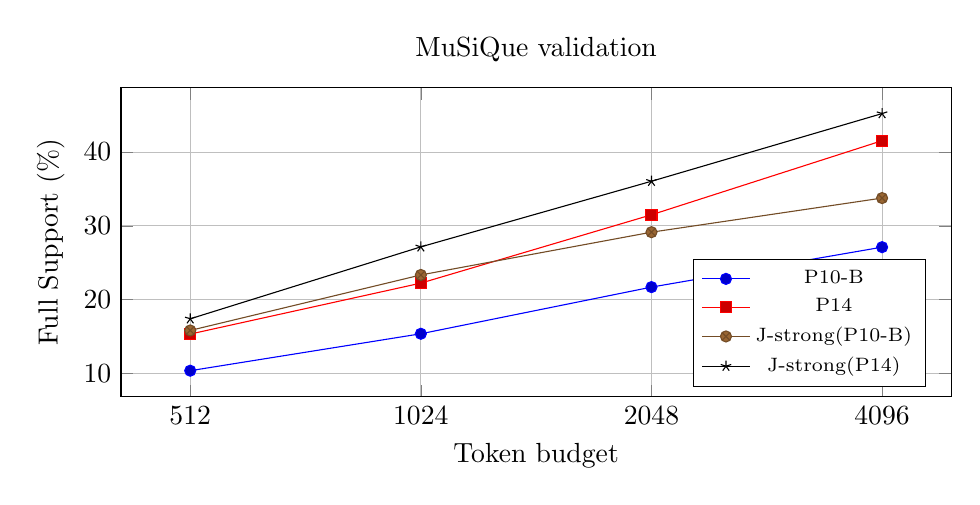
\begin{tikzpicture}
\begin{axis}[width=\columnwidth, height=5.5cm, xmode=log, log basis x=2, xtick={512,1024,2048,4096}, xticklabels={512,1024,2048,4096}, xlabel={Token budget}, ylabel={Full Support (\%)}, grid=major, legend pos=south east, legend style={font=\scriptsize}, title={MuSiQue validation}]
\addplot coordinates {(512,10.34) (1024,15.35) (2048,21.68) (4096,27.10)};
\addlegendentry{P10-B}
\addplot coordinates {(512,15.31) (1024,22.22) (2048,31.49) (4096,41.54)};
\addlegendentry{P14}
\addplot coordinates {(512,15.80) (1024,23.33) (2048,29.13) (4096,33.76)};
\addlegendentry{J-strong(P10-B)}
\addplot coordinates {(512,17.38) (1024,27.14) (2048,36.04) (4096,45.22)};
\addlegendentry{J-strong(P14)}
\end{axis}
\end{tikzpicture}
